\documentclass[12pt]{article}

\usepackage[a4paper, margin=1in]{geometry}
\usepackage{array}
\usepackage{multirow}
\usepackage{setspace}
\usepackage{graphicx}
\usepackage{float}
\usepackage{amssymb, amsmath, amsfonts}
\usepackage{enumitem}
\usepackage{listings}

\begin{document}

\begin{center}
    \textbf{\Large GATE Computer Science and Information Technology}
\end{center}

\vspace{0.3cm}

\noindent \textbf{\underline{General Aptitude}}

\vspace{0.3cm}

\noindent
\textbf{Q.1 -- Q.5 Carry ONE mark Each}

\vspace{0.5cm}

\renewcommand{\arraystretch}{1.8}

\begin{tabular}{|p{1.5cm}|p{12cm}|}
\hline

\textbf{Q.1} &
Expedite, Hasten, Hurry, \rule{3cm}{0.4pt}

\vspace{0.3cm}

Fill the blank by choosing a word with a meaning similar to the words above.
\\
\hline

(A) & Accelerate \\
\hline

(B) & Retard \\
\hline

(C) & Provide \\
\hline

(D) & Disable \\
\hline

\end{tabular}

\vspace{0.5cm}

\renewcommand{\arraystretch}{1.8}

\begin{tabular}{|p{1.5cm}|p{12cm}|}
\hline

\textbf{Q.2} &
A black square PQRS has been cut into two parts.

\vspace{0.2cm}

\begin{center}
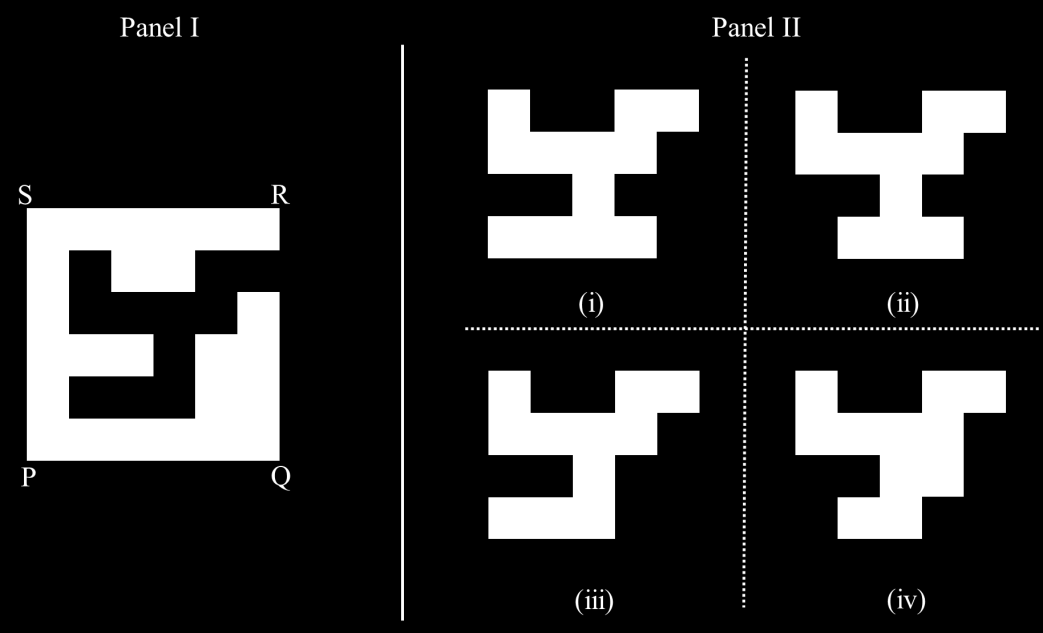
\includegraphics[width=0.4\textwidth]{figures/images-007.png}
\end{center}
\\

\hline

(A) & (i) \\
\hline

(B) & (ii) \\
\hline

(C) & (iii) \\
\hline

(D) & (iv) \\
\hline

\end{tabular}
\vspace{0.5cm}

\renewcommand{\arraystretch}{1.8}

\newpage

\begin{tabular}{|p{1.5cm}|p{12cm}|}
\hline

\textbf{Q.3} &
A day can only be cloudy or sunny. The probability of a day being cloudy is 0.5, independent of the condition on other days. What is the probability that in any given four days, there will be three cloudy days and one sunny day?
\\

\hline
(A) & 1/4 \\
\hline
(B) & 3/4 \\
\hline
(C) & 2/3 \\
\hline
(D) & 3/8 \\
\hline

\end{tabular}

\vspace{0.5cm}

\begin{tabular}{|p{1.5cm}|p{12cm}|}
\hline

\textbf{Q.4} &
The values of Stock A and Stock B on a particular day are Rs. 50 and Rs. 80, respectively. An investor invests Rs. 100 in Stock A and Rs. 80 in Stock B. He sells all the stocks the next day when the value of Stock A is Rs. 55 and Stock B is Rs. 70. The profit made by the investor is Rs. \_\_\_\_\_\_\_\_
\\

\hline
(A) & 0 \\
\hline
(B) & 5 \\
\hline
(C) & 10 \\
\hline
(D) & 20 \\
\hline

\end{tabular}

\vspace{0.5cm}

\begin{tabular}{|p{1.5cm}|p{12cm}|}
\hline

\textbf{Q.5} &
`When it is raining, peacocks dance.'

Based only on this sentence, which one of the following options is necessarily true?
\\

\hline
(A) & Peacocks dance only when it is raining. \\
\hline
(B) & When peacocks dance, it is raining. \\
\hline
(C) & When peacocks are not dancing, it is not raining. \\
\hline
(D) & When it is not raining, peacocks do not dance. \\
\hline

\end{tabular}
\newpage

\begin{tabular}{|p{1.5cm}|p{12cm}|}
\hline

\multicolumn{2}{|l|}{\textbf{Q.6 -- Q.10 Carry TWO marks Each}} \\
\hline

\textbf{Q.6} &
Water : P :: Food : Q

Choose the P and Q combination from the options below to form a meaningful analogy.
\\

\hline
(A) & P = Thirst; Q = Hunger \\
\hline
(B) & P = Drink; Q = Hunger \\
\hline
(C) & P = Thirst; Q = Satiated \\
\hline
(D) & P = Wet; Q = Critic \\
\hline

\end{tabular}

\vspace{0.7cm}

\begin{tabular}{|p{1.5cm}|p{12cm}|}
\hline

\textbf{Q.7} &
Two tiles are missing in Panel I. Which one of the options in Panel II is the appropriate choice for the missing tiles?
\\

\hline

\multicolumn{2}{|c|}{
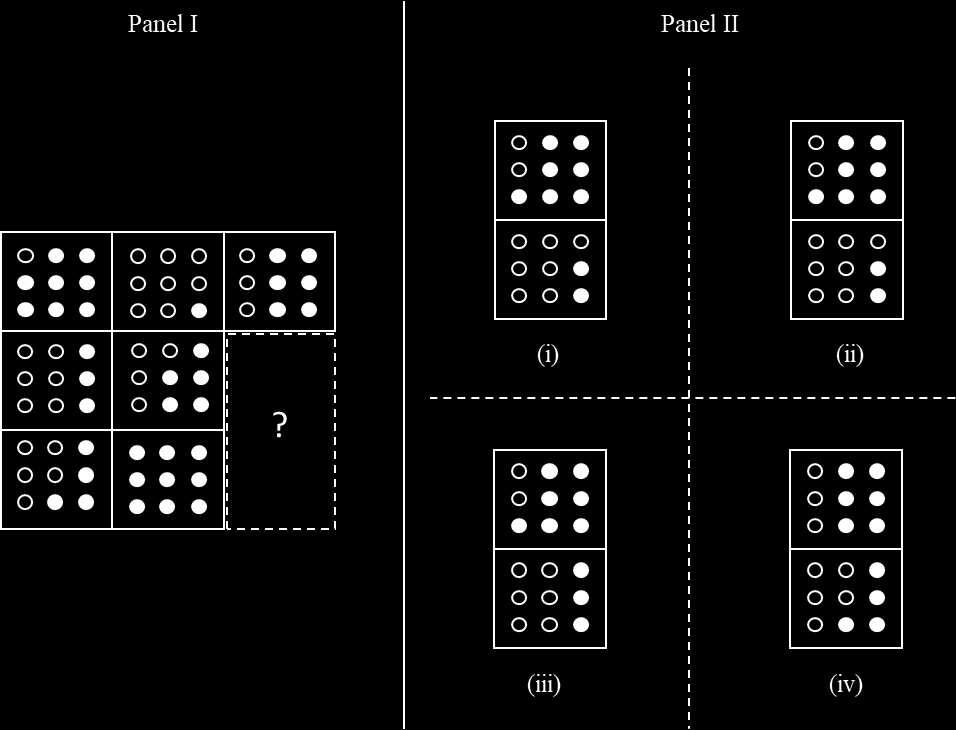
\includegraphics[width=0.75\textwidth]{figures/images-021.png}
}
\\

\hline

(A) & (i) \\
\hline
(B) & (ii) \\
\hline
(C) & (iii) \\
\hline
(D) & (iv) \\
\hline

\end{tabular}

\newpage

\begin{tabular}{|p{1.5cm}|p{12cm}|}
\hline

\textbf{Q.8} &
Three different views of a dice are shown below.

\begin{center}
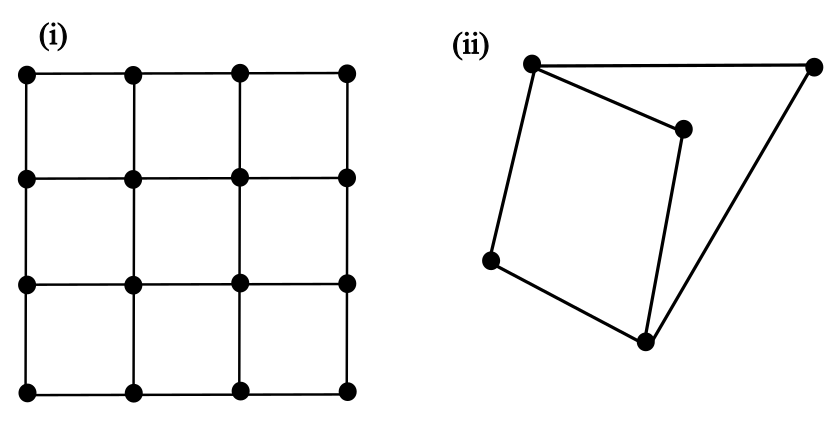
\includegraphics[width=0.45\textwidth]{figures/images-025.png}
\end{center}

If the face having number 1 is at the bottom, then the number on the top face is:
\\

\hline

(A) & 2 \\
\hline

(B) & 3 \\
\hline

(C) & 5 \\
\hline

(D) & 6 \\
\hline

\end{tabular}

\begin{tabular}{|p{1.5cm}|p{12cm}|}
\hline

\textbf{Q.9} &
A cube is shown with its dimensions.

\begin{center}
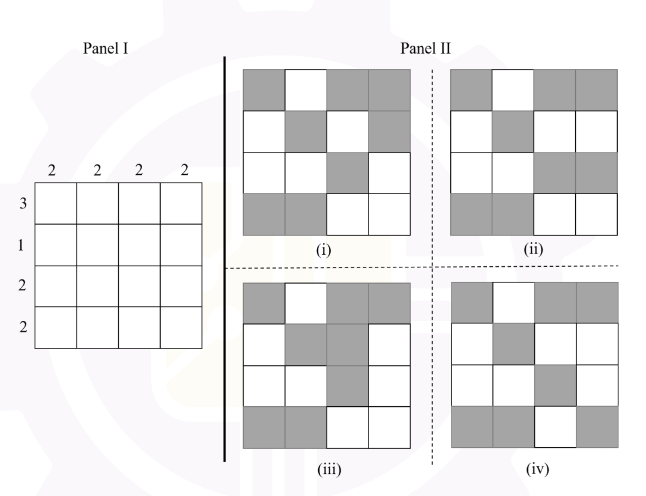
\includegraphics[width=0.55\textwidth]{figures/q9full.png}
\end{center}

Based on the above figures, identify the correct option.
\\

\hline

(A) & Only statement I is correct \\
\hline

(B) & Only statement II is correct \\
\hline

(C) & Both statements are correct \\
\hline

(D) & Neither statement is correct \\
\hline

\end{tabular}

\newpage

\begin{tabular}{|p{1.5cm}|p{12cm}|}
\hline

\textbf{Q.10} &
An unbiased six-faced dice whose faces are marked with numbers 1, 2, 3, 4, 5, and 6 is rolled twice in succession and the number on the top face is recorded each time. The probability that the sum of the two recorded numbers is a prime number is \_\_\_\_\_\_\_\_
\\

\hline

(A) & $\dfrac{3}{36}$ \\
\hline

(B) & $\dfrac{13}{36}$ \\
\hline

(C) & $\dfrac{15}{36}$ \\
\hline

(D) & $\dfrac{19}{36}$ \\
\hline

\end{tabular}

\vspace{0.9cm}

\noindent \textbf{Q.11 -- Q.35 Carry ONE mark Each}

\vspace{0.7cm}

\begin{tabular}{|p{1.2cm}|p{12cm}|}
\hline

\textbf{Q.11} &
For two different persons $x$ and $y$, the predicate $M(x,y)$ denotes that $x$ knows $y$.
Consider the following statement.

\vspace{0.7cm}

\textit{There is a person who does not know anyone else, but that person is known by everyone else.}

\vspace{0.5cm}

Which one of the following expressions represents the above statement?
\\

\hline

(A) & $(\exists y)(\forall x)\ ((x \neq y)\rightarrow(M(x,y)\wedge \neg M(y,x)))$ \\
\hline

(B) & $(\forall y)(\exists x)\ ((x \neq y)\rightarrow(M(x,y)\wedge \neg M(y,x)))$ \\
\hline

(C) & $(\exists y)(\exists x)\ ((x \neq y)\rightarrow(M(x,y)\wedge \neg M(y,x)))$ \\
\hline

(D) & $(\forall y)(\forall x)\ ((x \neq y)\rightarrow(M(x,y)\wedge \neg M(y,x)))$ \\
\hline

\end{tabular}

\vspace{0.5cm}

\begin{tabular}{|p{1.2cm}|p{12cm}|}
\hline

\textbf{Q.12} &
The set T represents various traversals over binary tree. The set S represents the order of visiting nodes during a traversal.

\vspace{0.4cm}

\begin{center}

\begin{tabular}{|c|c|}
\hline

\textbf{T} & \textbf{S} \\
\hline

I: Inorder & L: left subtree, node, right subtree \\
\hline

II: Preorder & M: node, left subtree, right subtree \\
\hline

III: Postorder & N: left subtree, right subtree, node \\
\hline

\end{tabular}

\end{center}

\vspace{0.3cm}

Which one of the following is the correct match from T to S ?
\\

\hline

(A) & I -- L, II -- M, III -- N \\
\hline

(B) & I -- M, II -- L, III -- N \\
\hline

(C) & I -- N, II -- M, III -- L \\
\hline

(D) & I -- L, II -- N, III -- M \\
\hline

\end{tabular}

\vspace{0.7cm}

\begin{tabular}{|p{1.2cm}|p{12cm}|}
\hline

\textbf{Q.13} &
Which one of the following statements is equivalent to the following assertion?

\vspace{0.3cm}

\begin{center}
Turing machine $M$ decides the language $L \subseteq \{0,1\}^{*}$
\end{center}
\\

\hline

(A) & Turing machine $M$ halts on all input strings in $\{0,1\}^{*}$ \\
\hline

(B) & Turing machine $M$ accepts all input strings in $L$ \\
\hline

(C) & Turing machine $M$ rejects all input strings in $\{0,1\}^{*} - L$ \\
\hline

(D) & Turing machine $M$ accepts all input strings in $L$ and rejects all input strings in $\{0,1\}^{*} - L$ \\
\hline

\end{tabular}

\vspace{0.7cm}

\begin{tabular}{|p{1.2cm}|p{12cm}|}
\hline

\textbf{Q.14} &
The probability density function $f(x)$ of a random variable $X$ which takes real values is

\vspace{0.4cm}

\begin{center}

$f(x)=\dfrac{1}{3\sqrt{2\pi}}\ \exp\left(-\dfrac{x^2}{18}\right), \qquad x \in (-\infty,+\infty)$

\end{center}

\vspace{0.3cm}

Which one of the following statements is correct about the random variable $X$ ?
\\

\hline

(A) & $X$ is an exponential random variable \\
\hline

(B) & $X$ is a normal random variable \\
\hline

(C) & $X$ is a Poisson random variable \\
\hline

(D) & $X$ is a uniform random variable \\
\hline

\end{tabular}

\vspace{0.7cm}

\begin{tabular}{|p{1.2cm}|p{12cm}|}
\hline

\textbf{Q.15} &
In the context of DBMS, consider the two sets T and S given below.

\vspace{0.4cm}

\begin{center}

\begin{tabular}{|c|c|}
\hline

\textbf{T} & \textbf{S} \\
\hline

I: Logical schema & L: Views \\
\hline

II: Physical schema & M: File organization and indexes \\
\hline

III: External schema & N: Relations \\
\hline

\end{tabular}

\end{center}

\vspace{0.3cm}

Which one of the following is the correct match from T to S ?
\\

\hline

(A) & I -- L, II -- M, III -- N \\
\hline

(B) & I -- M, II -- L, III -- N \\
\hline

(C) & I -- N, II -- M, III -- L \\
\hline

(D) & I -- N, II -- L, III -- M \\
\hline

\end{tabular}

\newpage

\begin{tabular}{|p{1.2cm}|p{12cm}|}
\hline

\textbf{Q.16} &
Which one of the following options is not a property of Boolean Algebra?

\vspace{0.3cm}

\textit{Note: + is OR operation, . is AND operation, and $'$ is NOT operation}
\\

\hline

(A) & $a+b=b+a$ \\
\hline

(B) & $a.a'=1$ \\
\hline

(C) & $a+a'=1$ \\
\hline

(D) & $a.b=b.a$ \\
\hline

\end{tabular}

\vspace{0.8cm}

\begin{tabular}{|p{1.2cm}|p{12cm}|}
\hline

\textbf{Q.17} &
In C runtime environment, which one of the following is stored in heap?
\\

\hline

(A) & A static variable declared inside a function \\
\hline

(B) & An array of integers declared inside a function \\
\hline

(C) & A dynamically allocated array of integers created using \texttt{malloc()} function call \\
\hline

(D) & Return address of a function \\
\hline

\end{tabular}

\vspace{0.8cm}

\begin{tabular}{|p{1.2cm}|p{12cm}|}
\hline

\textbf{Q.18} &
Consider the following two statements about interrupt handling mechanisms in a CPU.

\vspace{0.3cm}

\textbf{S1:} In non-vectored interrupt mechanism, it usually takes more time to start the Interrupt Service Routine (ISR) when compared to that in a vectored interrupt mechanism.

\vspace{0.3cm}

\textbf{S2:} In daisy-chain interrupt mechanism, the CPU polls all the input devices individually to determine the source of the interrupt.

\vspace{0.3cm}

Which one of the following options is correct with respect to S1 and S2 ?
\\

\hline

(A) & Both S1 and S2 are true \\
\hline

(B) & Both S1 and S2 are false \\
\hline

(C) & S1 is true and S2 is false \\
\hline

(D) & S1 is false and S2 is true \\
\hline

\end{tabular}

\newpage

\begin{tabular}{|p{1.2cm}|p{12cm}|}
\hline

\textbf{Q.19} &
Consider the following three ANSI-C programs, P1, P2, and P3.

\vspace{0.3cm}

{\scriptsize
\begin{center}
\begin{tabular}{|p{3.5cm}|p{3.5cm}|p{3.5cm}|}
\hline
\centering P1 & \centering P2 & \centering P3 \tabularnewline
\hline

{\ttfamily
\#include <stdio.h>

\vspace{0.2cm}

int a=5;

\vspace{0.2cm}

int main()\{

\quad int a=7;

\quad return(0);

\}
}
&
{\ttfamily
\#include <stdio.h>

\vspace{0.2cm}

int main()\{

\quad int a=5;

\quad int a=7;

\quad return(0);

\}
}
&
{\ttfamily
\#include <stdio.h>

\vspace{0.2cm}

int main()\{

\quad int a=5;

\quad float a=7;

\quad return(0);

\}
}
\\
\hline
\end{tabular}
\end{center}
}

\vspace{0.3cm}

Which one of the following statements is true?
\\
\hline

& \\
\hline

(A) & Only P1 will compile without any error \\
\hline

(B) & Only P2 will compile without any error \\
\hline

(C) & Only P3 will compile without any error \\
\hline

(D) & All three programs P1, P2, and P3 will compile without any error \\
\hline

\end{tabular}

\begin{tabular}{|p{1.2cm}|p{12cm}|}
\hline

\textbf{Q.20} &
Consider concurrent execution of two transactions $T1$ and $T2$ in a DBMS, both of which access a data object $A$. For these two transactions to not conflict on $A$, which one of the following statements must be true?
\\

\hline

(A) & Both $T1$ and $T2$ only read $A$ \\
\hline

(B) & $T1$ reads $A$ and $T2$ writes $A$ \\
\hline

(C) & $T1$ writes $A$ and $T2$ reads $A$ \\
\hline

(D) & Both $T1$ and $T2$ write $A$ \\
\hline

\end{tabular}

\newpage

\begin{tabular}{|p{1.5cm}|p{12cm}|}
\hline

Q.21 &
\parbox[t]{\linewidth}{
Consider a file of size 4 million bytes being transferred between two hosts connected via a path consisting of three consecutive links of bandwidth 2 Mbps, 500 kbps, and 1 Mbps, respectively. All processing delays and propagation delays are negligible. Assume that there is no other background traffic over the path and no other additional overhead to transfer the file.

\vspace{0.2cm}

Which one of the following is the total time (in seconds) to transfer the file?

\vspace{0.2cm}

\textit{Note:} $1M=10^6,\ 1k=10^3$
}
\\
\hline

(A) & 731 \\
\hline
(B) & 64 \\
\hline
(C) & 8 \\
\hline
(D) & 16 \\
\hline

\end{tabular}

\vspace{0.3cm}

\begin{tabular}{|p{1.5cm}|p{12cm}|}
\hline
Q.22 & Which one of the following protocols may need to broadcast some of its messages? \\
\hline
& \\
\hline
(A) & SMTP \\
\hline
(B) & FTP \\
\hline
(C) & DHCP \\
\hline
(D) & HTTP \\
\hline
\end{tabular}

\vspace{0.3cm}

\begin{tabular}{|p{1.5cm}|p{12cm}|}
\hline
Q.23 & Which one of the following CPU scheduling algorithms \textbf{cannot} be preemptive? \\
\hline
& \\
\hline
(A) & Shortest Remaining Time First (SRTF) Scheduling \\
\hline
(B) & First Come First Serve (FCFS) Scheduling \\
\hline
(C) & Round Robin Scheduling \\
\hline
(D) & Priority Scheduling \\
\hline
\end{tabular}

\newpage

\begin{tabular}{|p{1.5cm}|p{12cm}|}
\hline
Q.24 &
\parbox[t]{\linewidth}{
Consider the following functions, where $n$ is a positive integer.

\[
n^{1/3},\ \log(n),\ \log(n!),\ 2^{\log(n)}
\]

Which one of the following options lists the functions in increasing order of asymptotic growth rate?

\vspace{0.2cm}

\textit{Note:} Assume the base of log to be 2.
}
\\
\hline
& \\
\hline
(A) & $\log(n),\ n^{1/3},\ 2^{\log(n)},\ \log(n!)$ \\
\hline
(B) & $n^{1/3},\ \log(n),\ \log(n!),\ 2^{\log(n)}$ \\
\hline
(C) & $\log(n),\ n^{1/3},\ \log(n!),\ 2^{\log(n)}$ \\
\hline
(D) & $2^{\log(n)},\ n^{1/3},\ \log(n),\ \log(n!)$ \\
\hline
\end{tabular}

\vspace{0.3cm}

\begin{tabular}{|p{1.5cm}|p{12cm}|}
\hline
Q.25 &
Which of the following can be recurrence relation(s) corresponding to an algorithm with time complexity $\theta(n)$?
\\
\hline
& \\
\hline
(A) & $T(n)=T(n-1)+1,\qquad T(1)=1$ \\
\hline
(B) & $T(n)=2T\!\left(\frac{n}{2}\right)+1,\qquad T(1)=1$ \\
\hline
(C) & $T(n)=2T\!\left(\frac{n}{2}\right)+n,\qquad T(1)=1$ \\
\hline
(D) & $T(n)=T(n-1)+n,\qquad T(1)=1$ \\
\hline
\end{tabular}

\vspace{0.3cm}

\begin{tabular}{|p{1.5cm}|p{12cm}|}
\hline
Q.26 &
\parbox[t]{\linewidth}{
Let $R$ be a binary relation on the set $\{1,2,\ldots,10\}$, where $(x,y)\in R$ if the product of $x$ and $y$ is square of an integer. Which of the following properties is/are satisfied by $R$?
}
\\
\hline
& \\
\hline
(A) & Reflexive \\
\hline
(B) & Symmetric \\
\hline
(C) & Transitive \\
\hline
(D) & Antisymmetric \\
\hline
\end{tabular}

\newpage

\begin{tabular}{|p{1.5cm}|p{12cm}|}
\hline
Q.27 &
For a real number $a$, let
\[
I(a)=\int_{-1}^{1}(3x^2-ax+1)\,dx .
\]
Which of the following statements is/are true?
\\
\hline
& \\
\hline
(A) & The value of $I(a)$ is independent of the value of $a$ \\
\hline
(B) & The value of $I(a)$ can vary with the value of $a$ \\
\hline
(C) & There exists $a\in(-\infty,+\infty)$ such that $I(a)$ is a positive real number \\
\hline
(D) & There exists $a\in(-\infty,+\infty)$ such that $I(a)$ is a negative real number \\
\hline
\end{tabular}

\vspace{0.3cm}

\begin{tabular}{|p{1.5cm}|p{12cm}|}
\hline
Q.28 &
\parbox[t]{\linewidth}{
In a system, numbers are represented using 4-bit two's complement form. Consider four numbers $N1=1011$, $N2=1101$, $N3=1010$ and $N4=1001$ in the system. Which of the following operations will result in arithmetic overflow?
}
\\
\hline
& \\
\hline
(A) & $N1+N2$ \\
\hline
(B) & $N2+N3$ \\
\hline
(C) & $N3-N4$ \\
\hline
(D) & $N1+N4$ \\
\hline
\end{tabular}

\vspace{0.3cm}

\begin{tabular}{|p{1.5cm}|p{12cm}|}
\hline
Q.29 &
Which of the following grammars is/are ambiguous?
\\
\hline
& \\
\hline
(A) & $S \rightarrow aSb \mid \epsilon$ \\
\hline
(B) & $E \rightarrow E+E \mid E*E \mid id$ \\
\hline
(C) & $S \rightarrow aS \mid Sa \mid \epsilon$ \\
\hline
(D) & $S \rightarrow aS \mid \epsilon$ \\
\hline
\end{tabular}

\vspace{0.3cm}

\begin{tabular}{|p{1.5cm}|p{12cm}|}
\hline
Q.30 &
\parbox[t]{\linewidth}{
The keys 5, 28, 19, 15, 26, 33, 12, 17, 10 are inserted into a hash table using the hash function

\[
h(k)=k \bmod 9
\]

The collisions are resolved by chaining. After all the keys are inserted, the length of the longest chain is \rule{2cm}{0.15mm}. \textit{(answer in integer)}
}
\\
\hline
\end{tabular}

\vspace{0.3cm}

\begin{tabular}{|p{1.5cm}|p{12cm}|}
\hline
Q.31 &
\parbox[t]{\linewidth}{
Consider the system of linear equations given below.

\[
ax+y=b
\]

\[
16x+ay=24
\]

Suppose the values of $a$ and $b$ are chosen such that the system of linear equations produce multiple solutions. Then the product of $a$ and $b$ is \rule{2cm}{0.15mm}. \textit{(answer in integer)}
}
\\
\hline
\end{tabular}

\vspace{0.3cm}

\begin{tabular}{|p{1.5cm}|p{12cm}|}
\hline
Q.32 &
\parbox[t]{\linewidth}{
Consider an array

\[
A=[10,\ 7,\ 8,\ 19,\ 41,\ 35,\ 25,\ 31].
\]

Suppose the merge sort algorithm is executed on array $A$ to sort it in increasing order. The merge sort algorithm will carry out a total of 7 merge operations.

\vspace{0.2cm}

A merge operation on sorted left array $L$ and sorted right array $R$ is said to be void if the output of the merge operation is the elements of array $L$ followed by the elements of array $R$.

\vspace{0.2cm}

The number of void merge operations among these 7 merge operations is \rule{2cm}{0.15mm}. \textit{(answer in integer)}
}
\\
\hline
\end{tabular}

\vspace{0.3cm}

\begin{tabular}{|p{1.5cm}|p{12cm}|}
\hline
Q.33 &
If an IP network uses a subnet mask of 255.255.240.0, the maximum number of IP addresses that can be assigned to network interfaces is \rule{2cm}{0.15mm}. \textit{(answer in integer)}
\\
\hline
\end{tabular}

\vspace{0.3cm}

\begin{tabular}{|p{1.5cm}|p{12cm}|}
\hline
Q.34 &
\parbox[t]{\linewidth}{
The 32-bit IEEE 754 single precision representation of a number is

\[
\texttt{0xC2710000}.
\]

The number in decimal representation is \rule{2cm}{0.15mm}. \textit{(rounded off to two decimal places)}
}
\\
\hline
\end{tabular}

\vspace{0.3cm}

\begin{tabular}{|p{1.5cm}|p{12cm}|}
\hline
Q.35 &
\parbox[t]{\linewidth}{
A lexical analyzer uses the following token definitions

\[
\begin{aligned}
\textit{letter} &\rightarrow [A-Za-z] \\
\textit{digit} &\rightarrow [0-9] \\
\textit{id} &\rightarrow \textit{letter}\;(\textit{letter}\mid\textit{digit})^{*} \\
\textit{number} &\rightarrow \textit{digit}^{+} \\
\textit{ws} &\rightarrow (\textit{blank}\mid\textit{tab}\mid\textit{newline})^{+}
\end{aligned}
\]

For the string given below,

\[
\texttt{x1\ \ 23mm\ \ 78\ \ y\ \ 7z\ \ zz5\ \ 14A\ \ 8H\ \ AaYcD}
\]

the number of tokens (excluding \textit{ws}) that will be produced by the lexical analyzer is
\rule{2cm}{0.15mm}. \textit{(answer in integer)}
}
\\
\hline
\end{tabular}

\newpage

\textbf{Q.36 -- Q.65 Carry TWO marks Each}

\vspace{0.3cm}

\begin{tabular}{|p{1.5cm}|p{12cm}|}
\hline
Q.36 &
\parbox[t]{\linewidth}{
Consider a complete graph $K_n$ with $n$ vertices ($n>4$). Note that multiple spanning trees can be constructed over $K_n$. Each of these spanning trees is represented as a set of edges.

The Jaccard coefficient between any two sets is defined as the ratio of the size of the intersection of the two sets to the size of the union of the two sets.

Which one of the following options gives the lowest possible value for the Jaccard coefficient between any two spanning trees of $K_n$ ?
}
\\
\hline
& \\
\hline
(A) & $\dfrac{1}{n}$ \\
\hline
(B) & $\dfrac{1}{2n-3}$ \\
\hline
(C) & $0$ \\
\hline
(D) & $\dfrac{1}{n-1}$ \\
\hline
\end{tabular}

\vspace{0.3cm}

\begin{tabular}{|p{1.5cm}|p{12cm}|}
\hline
Q.37 &
\parbox[t]{\linewidth}{
Let $G$ be a weighted directed acyclic graph with $m$ edges and $n$ vertices.
Given $G$ and a source vertex $s$ in $G$, which one of the following options gives
the worst case time complexity of the fastest algorithm to find the lengths of
shortest paths from $s$ to all vertices that are reachable from $s$ in $G$?
}
\\
\hline
& \\
\hline
(A) & $\Theta(m+n)$ \\
\hline
(B) & $\Theta(m+n\log(n))$ \\
\hline
(C) & $\Theta(nm)$ \\
\hline
(D) & $\Theta(n^3)$ \\
\hline
\end{tabular}

\vspace{0.3cm}

\begin{tabular}{|p{1.5cm}|p{12cm}|}
\hline
Q.38 &
\parbox[t]{\linewidth}{
Consider an array $A$ of integers of size $n$. The indices of $A$ run from $1$ to $n$.
An algorithm is to be designed to check whether $A$ satisfies the condition given below.

\[
\forall i,j \in \{1,\ldots,n-1\}
\text{ such that } i>j,\;
(A[i+1]-A[i])>(A[j+1]-A[j])
\]

Which one of the following gives the worst case time complexity of the fastest
algorithm that can be designed for the problem?
}
\\
\hline
& \\
\hline
(A) & $\Theta(n)$ \\
\hline
(B) & $\Theta(\log(n))$ \\
\hline
(C) & $\Theta(n\log(n))$ \\
\hline
(D) & $\Theta(n^2)$ \\
\hline
\end{tabular}

\vspace{0.3cm}

\begin{tabular}{|p{1.5cm}|p{12cm}|}
\hline
Q.39 &
\parbox[t]{\linewidth}{
Consider a table $T$, where the elements $T[i][j]$, $0\le i,j\le n$,
represent the cost of the optimal solutions of different subproblems of a
problem that is being solved using a dynamic programming algorithm.

The recursive formulation to compute the table entries is as follows:

\[
T[0][k]=T[k][0]=1
\qquad \text{for } k=0,1,2,\ldots,n
\]

\[
T[i][j]=2T[i-1][j]+3T[i][j-1]
\qquad \text{for } 1\le i,j\le n
\]

Consider the following two algorithms to compute entries of $T$.
Assume that for both algorithms, for all $0\le i,j\le n$,
$T[i][j]$ has been initialized to $1$.

\vspace{0.2cm}

Algorithm $B_1$:

\[
\text{For } i=1,2,\ldots,n
\]

\[
\qquad \text{For } j=1,2,\ldots,n
\]

\[
\qquad\qquad T[i][j]=2T[i-1][j]+3T[i][j-1]
\]

\vspace{0.2cm}

Algorithm $B_2$:

\[
\text{For } s=2,3,\ldots,2n
\]

\[
\qquad \text{For } i=1,2,\ldots,n
\]

\[
\qquad\qquad \text{For } j=1,2,\ldots,n
\]

\[
\qquad\qquad\qquad \text{If } (i+j==s)
\]

\[
\qquad\qquad\qquad\qquad
T[i][j]=2T[i-1][j]+3T[i][j-1]
\]

\vspace{0.2cm}

Algorithm $B_k$, $k\in\{1,2\}$ is said to be correct if and only if it
calculates the correct values of $T[i][j]$, for all
$0\le i,j\le n$, (as per the recursive formulation) at the end of
the execution of the algorithm $B_k$.

Which one of the following statements is true?
}
\\
\hline
& \\
\hline
(A) & Both algorithms $B_1$ and $B_2$ are correct \\
\hline
(B) & Algorithm $B_1$ is correct, but algorithm $B_2$ is incorrect \\
\hline
(C) & Algorithm $B_2$ is correct, but algorithm $B_1$ is incorrect \\
\hline
(D) & Both algorithms $B_1$ and $B_2$ are incorrect \\
\hline
\end{tabular}

\vspace{0.3cm}

\begin{tabular}{|p{1.5cm}|p{12cm}|}
\hline
Q.40 &
\parbox[t]{\linewidth}{
Consider the following 4-variable Boolean function

\[
F(A,B,C,D)=\Sigma m(0,1,2,3,8,9,10,11)
\]

Consider $A$ as MSB, $D$ as LSB. Which one of the following options represents the minimal sum of products form for the above function?

\vspace{0.2cm}

\textit{Note:} $+$ is OR operation, $\cdot$ is AND operation, $'$ is NOT operation
}
\\
\hline
& \\
\hline
(A) & $A'+B'+C'+D'$ \\
\hline
(B) & $B'$ \\
\hline
(C) & $A'B'+AB$ \\
\hline
(D) & $A'$ \\
\hline
\end{tabular}

\vspace{0.3cm}

\begin{tabular}{|p{1.5cm}|p{12cm}|}
\hline
Q.41 &
\parbox[t]{\linewidth}{
Consider the canonical $LR(0)$ parsing of the grammar below using terminals $\{a,b,c\}$ and non-terminals $\{A,B,C,S\}$ with $S$ as the start symbol.

\[
S \rightarrow ACB
\]

\[
A \rightarrow aA \mid \epsilon
\]

\[
C \rightarrow cC \mid \epsilon
\]

\[
B \rightarrow bB \mid b
\]

Which one of the following options gives the number of shift-reduce conflicts that will occur in the $LR(0)$ ACTION table?
}
\\
\hline
& \\
\hline
(A) & 2 \\
\hline
(B) & 3 \\
\hline
(C) & 4 \\
\hline
(D) & 5 \\
\hline
\end{tabular}

\vspace{0.3cm}

\begin{tabular}{|p{1.5cm}|p{12cm}|}
\hline
Q.42 &
\parbox[t]{\linewidth}{
In the context of schema normalization in relational DBMS, consider a set $F$ of functional dependencies. The set of all functional dependencies implied by $F$ is called the closure of $F$.

To compute the closure of $F$, Armstrong's Axioms can be applied.

Consider $X,Y,$ and $Z$ as sets of attributes over a relational schema.

The three rules of Armstrong's Axioms are described as follows.

\vspace{0.2cm}

Reflexivity:
If $Y \subseteq X$, then $X \rightarrow Y$

\vspace{0.2cm}

Augmentation:
If $X \rightarrow Y$, then $XZ \rightarrow YZ$ for any $Z$

\vspace{0.2cm}

Transitivity:
If $X \rightarrow Y$ and $Y \rightarrow Z$, then $X \rightarrow Z$

\vspace{0.2cm}

The additional rule of Union is defined as follows.

\vspace{0.2cm}

Union:
If $X \rightarrow Y$ and $X \rightarrow Z$, then $X \rightarrow YZ$

\vspace{0.2cm}

It can be proved that the additional rule of Union is also implied by the three rules of Armstrong's Axioms.

Listed below are four combinations of these three rules.

Which one of these combinations is both necessary and sufficient for the proof?
}
\\
\hline
& \\
\hline
(A) & Reflexivity, Augmentation, and Transitivity \\
\hline
(B) & Reflexivity and Augmentation \\
\hline
(C) & Transitivity \\
\hline
(D) & Augmentation and Transitivity \\
\hline
\end{tabular}

\vspace{0.3cm}

\begin{tabular}{|p{1.5cm}|p{12cm}|}
\hline
Q.43 &
\parbox[t]{\linewidth}{
Consider the transmission of data bits 110001011 over a link that uses Cyclic Redundancy Check (CRC) code for error detection.

If the generator bit pattern is given to be 1001, which one of the following options shows the remainder bit pattern appended to the data bits before transmission?
}
\\
\hline
& \\
\hline
(A) & 011 \\
\hline
(B) & 101 \\
\hline
(C) & 000 \\
\hline
(D) & 100 \\
\hline
\end{tabular}

\vspace{0.3cm}

\begin{tabular}{|p{1.5cm}|p{12cm}|}
\hline
Q.44 &
\parbox[t]{\linewidth}{
Consider a processor that has 16 general purpose registers and it uses 2-byte instruction format for all its instructions.

Variable-sized opcodes are permitted.

There are three different types of instructions: M-type, R-type, and C-type.

Each M-type instruction has 2 register operands and a 6-bit immediate operand.

Each R-type instruction has 3 register operands.

Each C-type instruction has a register operand and a 6-bit offset value.

If there are 2 unique M-type opcodes and 7 unique R-type opcodes, which one of the following options gives the maximum number of unique opcodes possible for C-type instructions?
}
\\
\hline
& \\
\hline
(A) & 8 \\
\hline
(B) & 4 \\
\hline
(C) & 64 \\
\hline
(D) & 16 \\
\hline
\end{tabular}

\vspace{0.3cm}

\begin{tabular}{|p{1.5cm}|p{12cm}|}
\hline
Q.45 &
\parbox[t]{\linewidth}{
Consider the control flow graph given below.

\begin{center}
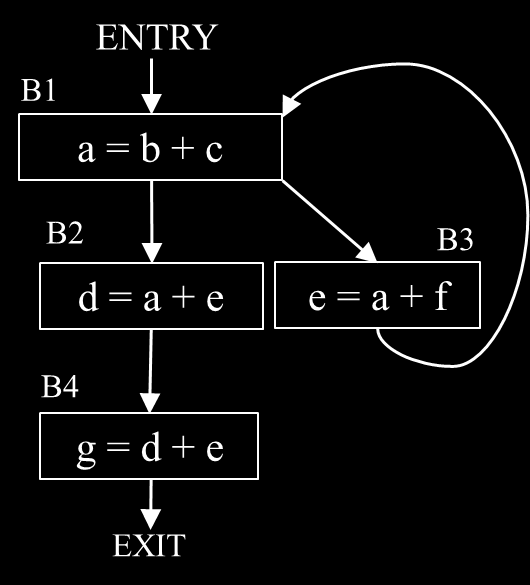
\includegraphics[width=0.55\textwidth]{./figures/images-101.png}
\end{center}

Which one of the following options is the set of live variables at the exit point of each basic block?
}
\\
\hline
& \\
\hline
(A) & B1:\{a,b,c,e,f\}, B2:\{d,e\}, B3:\{b,c,e,f\}, B4:$\emptyset$ \\
\hline
(B) & B1:$\emptyset$, B2:\{d,e\}, B3:\{a,c,f\}, B4:$\emptyset$ \\
\hline
(C) & B1:\{a,b,c,e,f\}, B2:\{d,e\}, B3:\{c,e,f\}, B4:$\emptyset$ \\
\hline
(D) & B1:$\emptyset$, B2:\{d,e,f\}, B3:\{a,b,c,e,f\}, B4:$\emptyset$ \\
\hline
\end{tabular}

\vspace{0.3cm}

\begin{tabular}{|p{1.5cm}|p{12cm}|}
\hline
Q.46 &
\parbox[t]{\linewidth}{
An index in a DBMS is said to be dense if an index entry appears for every search-key value in the indexed file. Otherwise it is called a sparse index. Consider the following two statements.

\vspace{0.2cm}

S1: A hash index must be a dense index

S2: A $B^{+}$ tree index can be a sparse index

\vspace{0.2cm}

Which one of the following options is correct?
}
\\
\hline
& \\
\hline
(A) & Both S1 and S2 are true \\
\hline
(B) & Both S1 and S2 are false \\
\hline
(C) & S1 is true and S2 is false \\
\hline
(D) & S1 is false and S2 is true \\
\hline
\end{tabular}

\vspace{0.3cm}

\begin{tabular}{|p{1.5cm}|p{12cm}|}
\hline
Q.47 &
\parbox[t]{\linewidth}{
Consider the following two finite automata $D_1$ and $D_2$.

\begin{center}
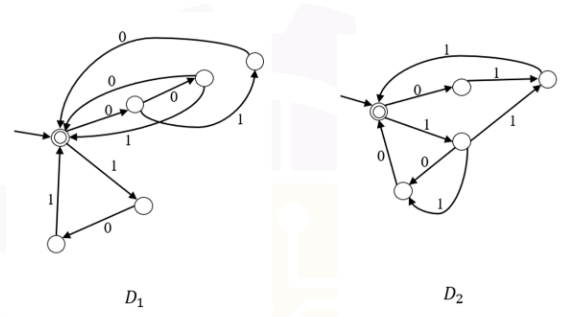
\includegraphics[width=\linewidth]{./figures/images-140.png}
\end{center}

Which of the following statements is/are true?
}
\\
\hline
& \\
\hline
(A) & $L(D_1)=L(D_2)$ \\
\hline
(B) & $L(D_1)$ is a proper subset of $L(D_2)$ \\
\hline
(C) & $L(D_1)\cap L(D_2)=\{\epsilon\}$ \\
\hline
(D) & $(L(D_1)\cup L(D_2))^*$ consists of all strings in $\{0,1\}^*$ whose length is divisible by $3$ \\
\hline
\end{tabular}

\vspace{0.3cm}

\begin{tabular}{|p{1.5cm}|p{12cm}|}
\hline
Q.48 &
\parbox[t]{\linewidth}{
Let $\Sigma=\{a,b,c,d\}$ and let

\[
L=\{a^i b^j c^k d^\ell \mid i,j,k,\ell \ge 0\}.
\]

Which of the following constraints ensure(s) that the language $L$ is context-free?
}
\\
\hline
& \\
\hline
(A) & $i+k=j+\ell$ \\
\hline
(B) & $i=k$ and $j=\ell$ \\
\hline
(C) & $i=\ell$ and $j=k$ \\
\hline
(D) & $i+j=k+\ell$ \\
\hline
\end{tabular}

\vspace{0.3cm}

\begin{tabular}{|p{1.5cm}|p{12cm}|}
\hline
Q.49 &
\parbox[t]{\linewidth}{
Consider a binary search tree (BST) with $n$ leaf nodes ($n>0$). Given any node $V$, the key present in the node is denoted as $Val(V)$. All the keys present in the given BST are distinct. The keys belong to the set of real numbers.

\vspace{0.2cm}

For a node $V$, let $Suc(V)$ denote the node that is its inorder successor. If a node $V$ does not have an inorder successor, then $Suc(V)$ is NULL. As there are no duplicates, if $Suc(V)$ is not NULL, then $Val(V)<Val(Suc(V))$.

\vspace{0.2cm}

Corresponding to every leaf node $L_i$ that has a non-NULL $Suc(L_i)$, a new key $k_i$ with the following property is to be inserted into the BST.

\[
Val(L_i)<k_i<Val(Suc(L_i))
\]

Let $K$ represent the list of all such new keys to be inserted into the BST.

\vspace{0.2cm}

Which of the following statements is/are true?
}
\\
\hline
& \\
\hline
(A) & $K$ cannot have any duplicates \\
\hline
(B) & $K$ will have at least one element \\
\hline
(C) & After inserting all keys from $K$, the height of the BST can increase at most by one \\
\hline
(D) & Number of nodes in the BST will double after inserting all keys from $K$ \\
\hline
\end{tabular}

\vspace{0.3cm}

\begin{tabular}{|p{1.5cm}|p{12cm}|}
\hline
Q.50 &
\parbox[t]{\linewidth}{
Consider a stack $S$ and a queue $Q$. Both of them are initially empty and have the capacity to store ten elements each. The elements $1,2,3,4,$ and $5$ arrive one by one, in that order. When an element arrives, it is assigned either to $S$ (pushed on $S$) or to $Q$ (enqueued to $Q$). Once all the five elements are stored, the output is generated in two steps. First, stack $S$ is emptied by popping all elements. Then queue $Q$ is emptied by dequeuing all elements. The output obtained by following this process is $4\ 3\ 1\ 2\ 5$.

\vspace{0.2cm}

Given the output, the objective is to predict whether an element was assigned to $S$ or $Q$.

\vspace{0.2cm}

\textit{Note: In the options, the notation xS denotes that element x was assigned to S and yQ denotes that element y was assigned to Q.}

\vspace{0.2cm}

Which of the following options is/are possible valid assignment(s) of the elements?
}
\\
\hline
& \\
\hline
(A) & 1S, 2Q, 3S, 4S, 5Q \\
\hline
(B) & 1Q, 2Q, 3S, 4S, 5Q \\
\hline
(C) & 1Q, 2Q, 3Q, 4S, 5S \\
\hline
(D) & 1S, 2S, 3S, 4Q, 5Q \\
\hline
\end{tabular}

\vspace{0.3cm}

\begin{tabular}{|p{1.5cm}|p{12cm}|}
\hline
Q.51 &
\parbox[t]{\linewidth}{
Consider three processes P1, P2, and P3 running identical code, as shown in the pseudocode below. A and B are two binary semaphores initialized to 1 and 0, respectively. X is a shared variable initialized to 0. Each line in the pseudocode is executed atomically.

\begin{center}
\begin{minipage}{0.55\linewidth}
\ttfamily
Wait(A);\\
Print(*);\\
X = X + 1;\\
If (X == 2)\\
\{\\
\hspace*{1cm}Print(\$);\\
\hspace*{1cm}Signal(B);\\
\}\\
Signal(A);\\
Wait(B);\\
Print(\#);\\
Signal(B);
\end{minipage}
\end{center}

Assume that any of the three processes can start to execute first and context switching can happen between these processes at any arbitrary time and in any arbitrary order.

\vspace{0.2cm}

Which of the following patterns is/are possible to be generated as an outcome of the execution of these three processes?
}
\\
\hline
& \\
\hline
(A) & \texttt{**\$*\#\#\#} \\
\hline
(B) & \texttt{**\$\#*\#\#} \\
\hline
(C) & \texttt{**\$\#\#*\#} \\
\hline
(D) & \texttt{***\$\#\#\#} \\
\hline
\end{tabular}

\vspace{0.3cm}

\begin{tabular}{|p{1.5cm}|p{12cm}|}
\hline
Q.52 &
\parbox[t]{\linewidth}{
Consider a system with a processor and a 4 KB direct mapped cache with block size of 16 bytes. The system has a 16 MB physical memory. Four words P, Q, R, and S are accessed by the processor in the same order 10 times. That is, there are a total of 40 memory references in the sequence P, Q, R, S, P, Q, R, S, \ldots

\vspace{0.2cm}

Assume that the cache memory is initially empty. The physical addresses of the words are given below (1 word = 1 byte).

\[
P: 0x845B32,\quad
Q: 0x845B26,\quad
R: 0x845B36,\quad
S: 0x846B32
\]

Which of the following statements is/are true?

\vspace{0.2cm}

\textit{Note: $1K=2^{10}$ and $1M=2^{20}$}
}
\\
\hline
& \\
\hline
(A) & Every access to P results in a cache miss \\
\hline
(B) & Every access to R results in a cache hit \\
\hline
(C) & Every access to Q results in a cache miss \\
\hline
(D) & Except the first access to S, all subsequent accesses to S result in cache hits \\
\hline
\end{tabular}

\vspace{0.3cm}

\begin{tabular}{|p{1.5cm}|p{12cm}|}
\hline
Q.53 &
\parbox[t]{\linewidth}{
To keep track of free blocks in a file system, one of the two approaches is generally used -- using bitmaps (bit vectors) or using linked lists. Consider that the linked list approach is used to keep track of free blocks in a file system. Assume that the disk size is 16 GB, block size is 2 KB, and block numbers used are 32-bit long. A single pointer of size 4 bytes is used in each block of the list to point to the next block of the list.

\vspace{0.2cm}

The number of blocks required to hold the free disk block numbers is \underline{\hspace{2cm}}. (\textit{answer in integer})

\vspace{0.2cm}

\textit{Note: $1K=2^{10}$ and $1G=2^{30}$}
}
\\
\hline
\end{tabular}

\vspace{0.3cm}

\begin{tabular}{|p{1.5cm}|p{12cm}|}
\hline
Q.54 &
\parbox[t]{\linewidth}{
A system has a Translation Lookaside Buffer (TLB) that has a reach of 1 MB. TLB reach is defined as the total amount of physical memory that can be accessed through the TLB entries. The paging system uses pages of size 4 KB. The virtual address space is 64 GB and physical address space is 1 GB. If each TLB entry stores a 4-bit process id, page number, frame number, and a 2-bit control field, then the size of the TLB (in bytes) is \underline{\hspace{2cm}}. \textit{(answer in integer)}

\vspace{0.2cm}

\textit{Note: 1K=$2^{10}$, 1M=$2^{20}$, 1G=$2^{30}$}
}
\\
\hline
\end{tabular}

\vspace{0.3cm}

\begin{tabular}{|p{1.5cm}|p{12cm}|}
\hline
Q.55 &
\parbox[t]{\linewidth}{
Consider contiguous allocation of physical memory to processes using variable partitioning scheme. Suppose there are 8 holes in the memory of sizes 20 KB, 4 KB, 25 KB, 18 KB, 7 KB, 9 KB, 15 KB, and 12 KB. Assume that no two holes are adjacent. Two processes P1 of size 16 KB and P2 of size 9 KB arrive in that order, and they are allocated memory using the best-fit technique. After allocating space to P1 and P2, the number of holes of size less than 8 KB is \underline{\hspace{2cm}}. \textit{(answer in integer)}

\vspace{0.2cm}

\textit{Note: 1K=$2^{10}$}
}
\\
\hline
\end{tabular}

\vspace{0.3cm}

\begin{tabular}{|p{1.5cm}|p{12cm}|}
\hline
Q.56 &
\parbox[t]{\linewidth}{
Consider a system with 1 MB physical memory and a word length of 1 byte. The system uses a direct mapped cache, with block numbers starting from 0. The word with physical address 0xA2C28 is mapped to the cache block number 176$_{10}$. The maximum possible size of the cache (in KB) for this configuration is \underline{\hspace{2cm}}. \textit{(answer in integer)}

\vspace{0.2cm}

\textit{Note: 1K=$2^{10}$ and 1M=$2^{20}$}
}
\\
\hline
\end{tabular}

\vspace{0.3cm}

\begin{tabular}{|p{1.5cm}|p{12cm}|}
\hline
Q.57 &
\parbox[t]{\linewidth}{
A non-pipelined instruction execution unit that operates at 1.6 GHz clock takes an average of 5 clock cycles to complete the execution of an instruction. To improve the performance, the system was pipelined with a goal of achieving an average throughput of one instruction per clock cycle. However, it could operate only at 1.2 GHz due to pipeline overheads. While executing a program in the pipelined design, 30\% of instructions encountered a stall of 2 cycles due to pipeline hazards. The speed-up obtained by the pipelined design over the non-pipelined one for this program is \underline{\hspace{2cm}}. \textit{(rounded off to two decimal places)}

\vspace{0.3cm}

\textit{Note: 1G=$10^9$}
}
\\
\hline
\end{tabular}

\vspace{0.3cm}

\begin{tabular}{|p{1.5cm}|p{12cm}|}
\hline
Q.58 &
\parbox[t]{\linewidth}{
Consider a new TCP connection between a sender and a receiver. The receiver advertised window is constant at 48 KB, the maximum segment size (MSS) is 2 KB, and the slow start threshold for TCP congestion control is 16 KB. Assume that there are no timeouts or duplicate acknowledgements. The number of rounds of transmission required for the congestion control algorithm of the TCP connection to reach the congestion avoidance phase is \underline{\hspace{2cm}}. \textit{(answer in integer)}

\vspace{0.3cm}

\textit{Note: $1K = 2^{10}$}
}
\\
\hline
\end{tabular}

\vspace{0.3cm}

\begin{tabular}{|p{1.5cm}|p{12cm}|}
\hline
Q.59 &
\parbox[t]{\linewidth}{
Consider the digital circuit shown below with two input lines A and B, two select lines S0 and S1, and an output line Y. The blocks Q and M represent active high 2:4 decoder and 4-to-1 multiplexer, respectively. Out of 16 possible input combinations, the number of combinations that produce Y=1 is \underline{\hspace{2cm}}. \textit{(answer in integer)}

\vspace{0.3cm}

\textit{Note: One input combination is an instance of [A B S1 S0].}

\begin{center}
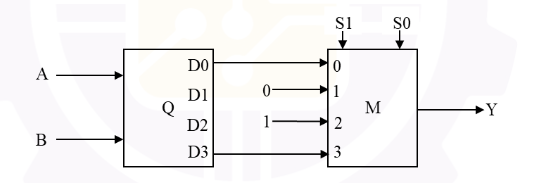
\includegraphics[width=0.55\textwidth]{./figures/images-143.png}
\end{center}
}
\\
\hline
\end{tabular}

\vspace{0.3cm}

\begin{tabular}{|p{1.5cm}|p{12cm}|}
\hline
Q.60 &
\parbox[t]{\linewidth}{
Consider the following ANSI-C program.

\vspace{0.3cm}

\ttfamily
\begin{flushleft}
\small
\#include <stdio.h>\\

int main()\{\\
\quad int *ptr, a, b, c;\\
\quad a=5; b=11; c=20;\\
\quad ptr=\&a; *ptr=c; ptr=\&c;\\
\quad a=* (\&b); c=*ptr-a;\\
\quad printf("\%d",c);\\
\quad return(0);\\
\}
\end{flushleft}
\normalfont

The output of this program is \underline{\hspace{2cm}}. \textit{(answer in integer)}

\vspace{0.3cm}

\textit{Note: Assume that the program compiles and runs successfully.}
}
\\
\hline
\end{tabular}

\vspace{0.3cm}

\begin{tabular}{|p{1.5cm}|p{12cm}|}
\hline
Q.61 &
\parbox[t]{\linewidth}{
Consider the following ANSI-C function.

\vspace{0.3cm}

{\ttfamily
int func(int start, int end)\{\\
\quad int length=end+1-start;\\
\quad if((length<1)||(start<0)||(end<0))\{ return(0); \}\\
\quad if(length\%3==0)\{\\
\qquad return(func(start+1,end));\\
\quad \}\\
\quad else if(length\%3==1)\{\\
\qquad return(1+func(start,end-1));\\
\quad \}\\
\quad else \{\\
\qquad return(func(start+2,end));\\
\quad \}\\
\}
}

The maximum possible value that can be returned from this function is \underline{\hspace{2cm}}. \textit{(answer in integer)}

\vspace{0.3cm}

\textit{Note: Ignore syntax errors (if any) in the function.}
}
\\
\hline
\end{tabular}

\vspace{0.3cm}

\begin{tabular}{|p{1.5cm}|p{12cm}|}
\hline
Q.62 &
\parbox[t]{\linewidth}{
The determinant of a $4 \times 4$ matrix $A$ is 3. The value of the determinant of $2A$ is \underline{\hspace{2cm}}. \textit{(answer in integer)}
}
\\
\hline
\end{tabular}

\vspace{0.3cm}

\begin{tabular}{|p{1.5cm}|p{12cm}|}
\hline
Q.63 &
\parbox[t]{\linewidth}{
Suppose an unbiased coin is tossed 6 times. Each coin toss is independent of all previous coin tosses. Let $E_1$ be the event that among the second, fourth, and sixth coin tosses, there are at least two heads. Let $E_2$ be the event that among the first, second, third, and fifth coin tosses, there are equal number of heads and tails.

\vspace{0.3cm}

The conditional probability $P(E_1|E_2)$ is equal to \underline{\hspace{2cm}}. \textit{(rounded off to one decimal place)}
}
\\
\hline
\end{tabular}


\vspace{0.3cm}

\begin{tabular}{|p{1.5cm}|p{12cm}|}
\hline
Q.64 &
\parbox[t]{\linewidth}{
Consider a function $f:(0,1)\rightarrow\{0,1\}$ defined as follows.

\vspace{0.3cm}

For a real number $r \in (0,1)$, $f(r)=1$ if the second digit after the decimal point in $r$ is one of the four digits 2, 3, 6 and 7. Otherwise, $f(r)$ is equal to 0.

\vspace{0.2cm}

The number of points in $(0,1)$ at which $f$ is discontinuous is \underline{\hspace{2cm}}. \textit{(answer in integer)}
}
\\
\hline
\end{tabular}

\vspace{0.3cm}

\begin{tabular}{|p{1.5cm}|p{12cm}|}
\hline
Q.65 &
\parbox[t]{\linewidth}{
It is necessary to design a link-layer protocol between two hosts that are directly connected over a lossless link of length 3000 kilometers. Assume that the link bandwidth is $10^8$ bits per second and that the propagation delay in the link is 5 nanoseconds per meter. Every transmitted data byte is assigned a unique sequence number.

\vspace{0.3cm}

Let $N$ be the minimum number of bits needed for the sequence number field in the protocol header such that

\begin{enumerate}
\item the sequence numbers do not wrap around before 60 seconds, and
\item the maximum utilization of the link is achieved.
\end{enumerate}

The value of $N$ is \underline{\hspace{2cm}}. \textit{(answer in integer)}
}
\\
\hline
\end{tabular}

\end{document}

